\documentclass[12pt]{article}
\usepackage[a4paper,bindingoffset=0.2in,left=2.5cm,right=2.5cm,top=1.5cm,bottom=1.5cm,footskip=.25in]{geometry}
\usepackage{graphicx}
\usepackage{caption}
\usepackage{subcaption}
\usepackage{placeins}
\usepackage{amsmath}

%================================
\title{Comparison of Angles from Gait Lab and EXL IMU Sensors after Interpolation of the data}
\author{}


\begin{document}
\maketitle


\section*{Comparison}

In the previous comparison of the results one of the problems that we faced is that an average step from the Gait Lab contains 100 sample points (may be this is after normalization) and ours contained 126 points, which made the graphs look something like this

\begin{figure}[!htb]
\centering
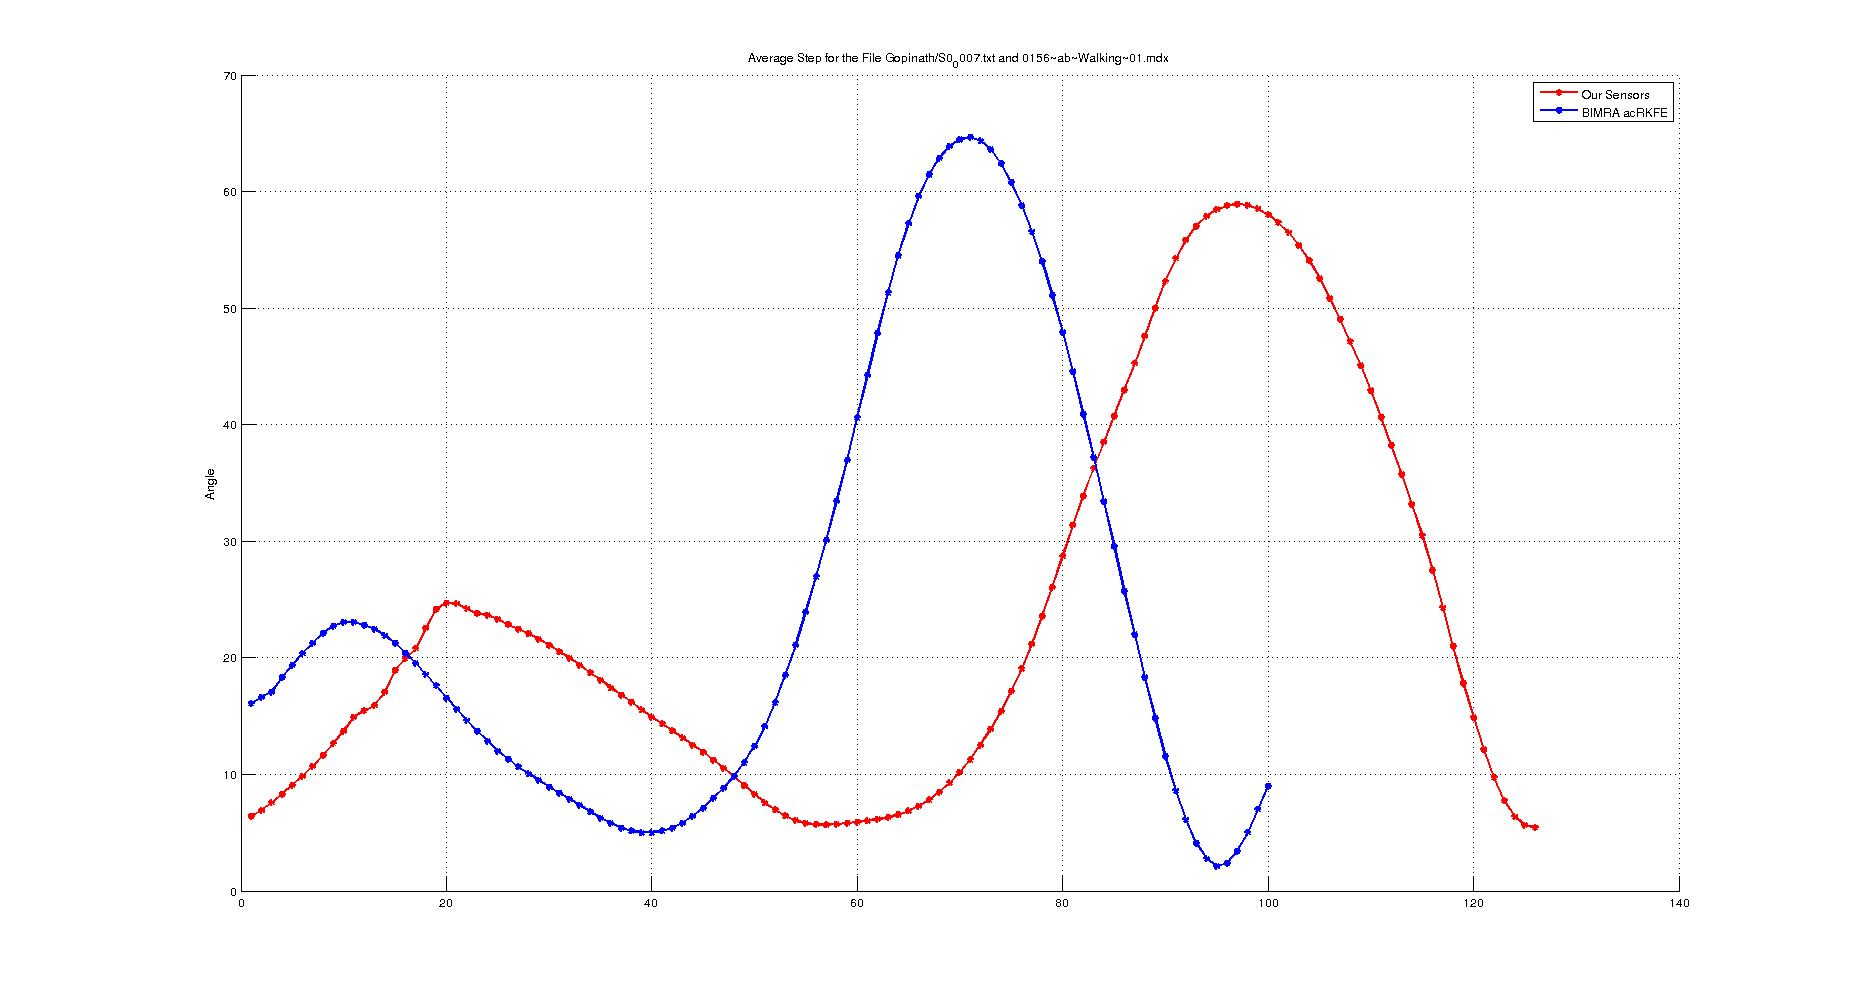
\includegraphics[scale=.25]{NormalCompareacRKFE.jpg}
\caption{Comparison of the Joint angle before Interpolation}
\label{acRKFEOld}
\end{figure}

\FloatBarrier

We can see that the data point of the GAIT Lab step stops much before the EXL IMU data points.\\

After Interpolating the GAIT Lab data to 126 points, using the matlab command:
\begin{verbatim}
	avgStepBimraInter = interp1(1:1:100, avgStepBimra, 1:100/127:100);
\end{verbatim}

the plot looks like.

\begin{figure}[!htb]
\centering
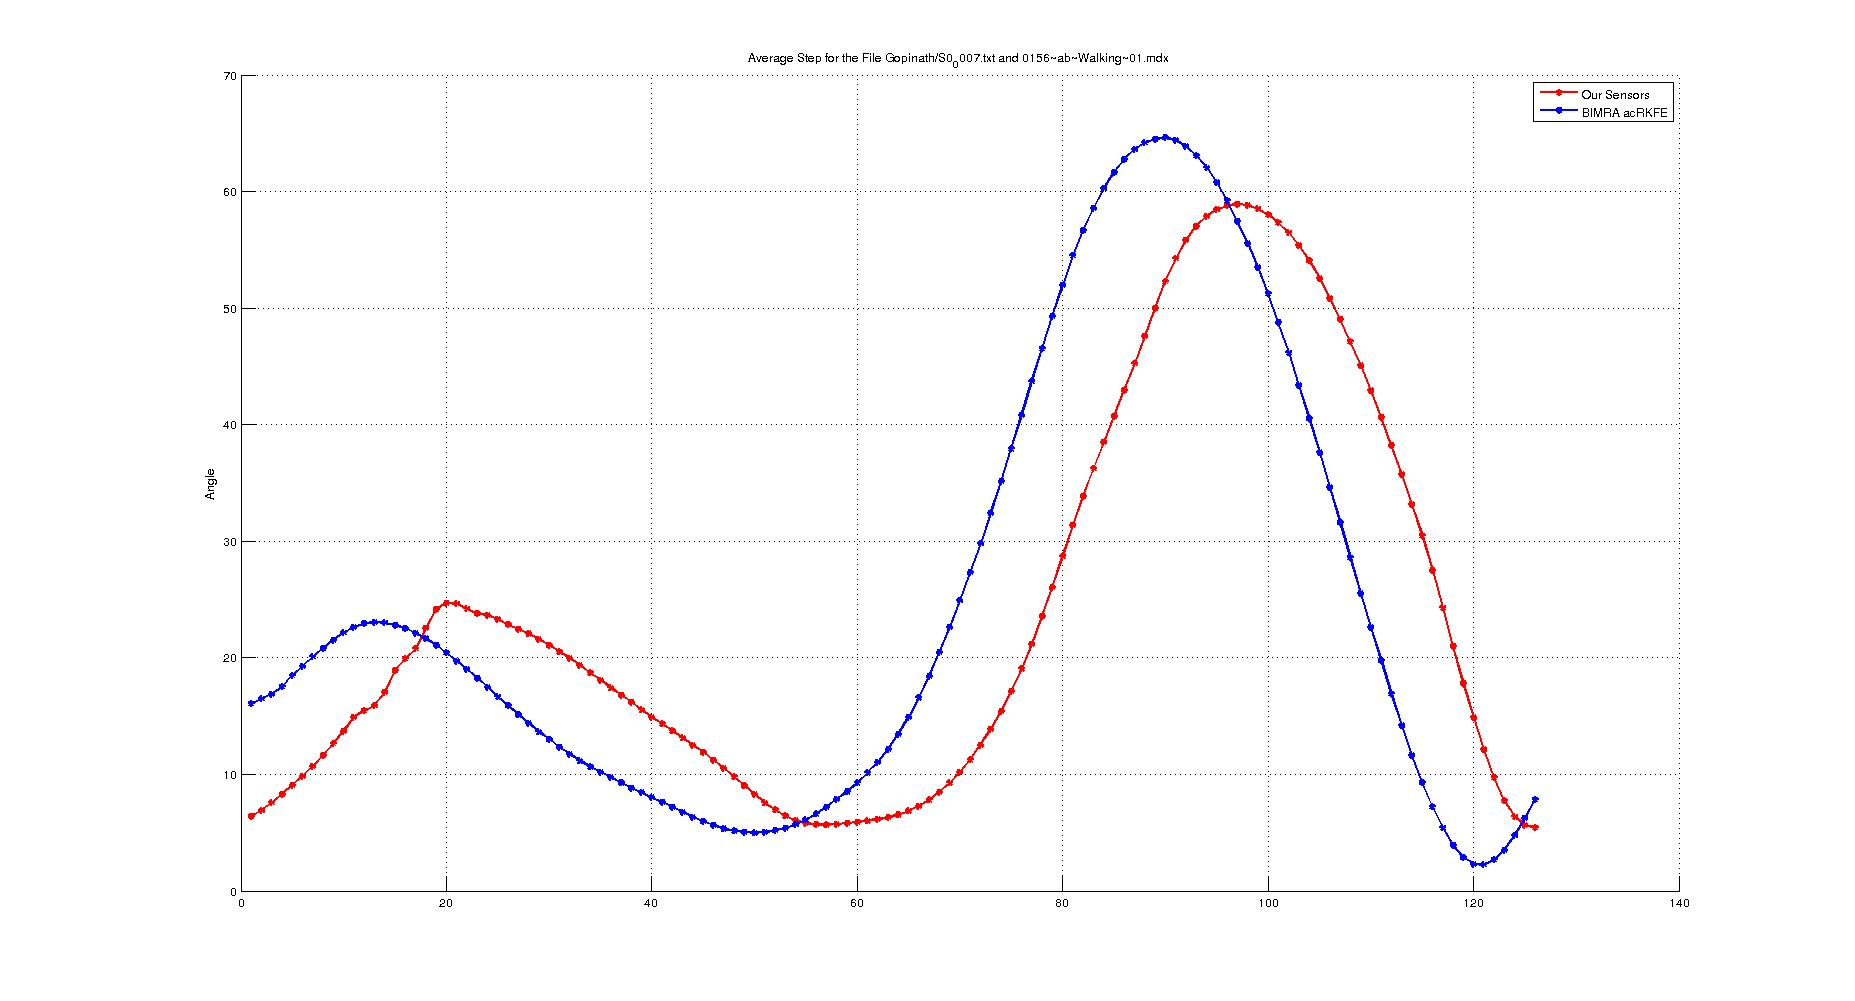
\includegraphics[scale=.25]{interPolatedCompareacRKFE.jpg}
\caption{Comparison of the Joint angle after Interpolation}
\label{acRKFENew}
\end{figure}

\FloatBarrier
Need to find a way to normalize the EXL IMU Steps to 100 points.

\FloatBarrier
\subsection*{Comparison of Rest of the Steps, using acRKFE}
\begin{figure}[h]%

\begin{subfigure}[!htb]{2cm}
\hspace*{-2cm} 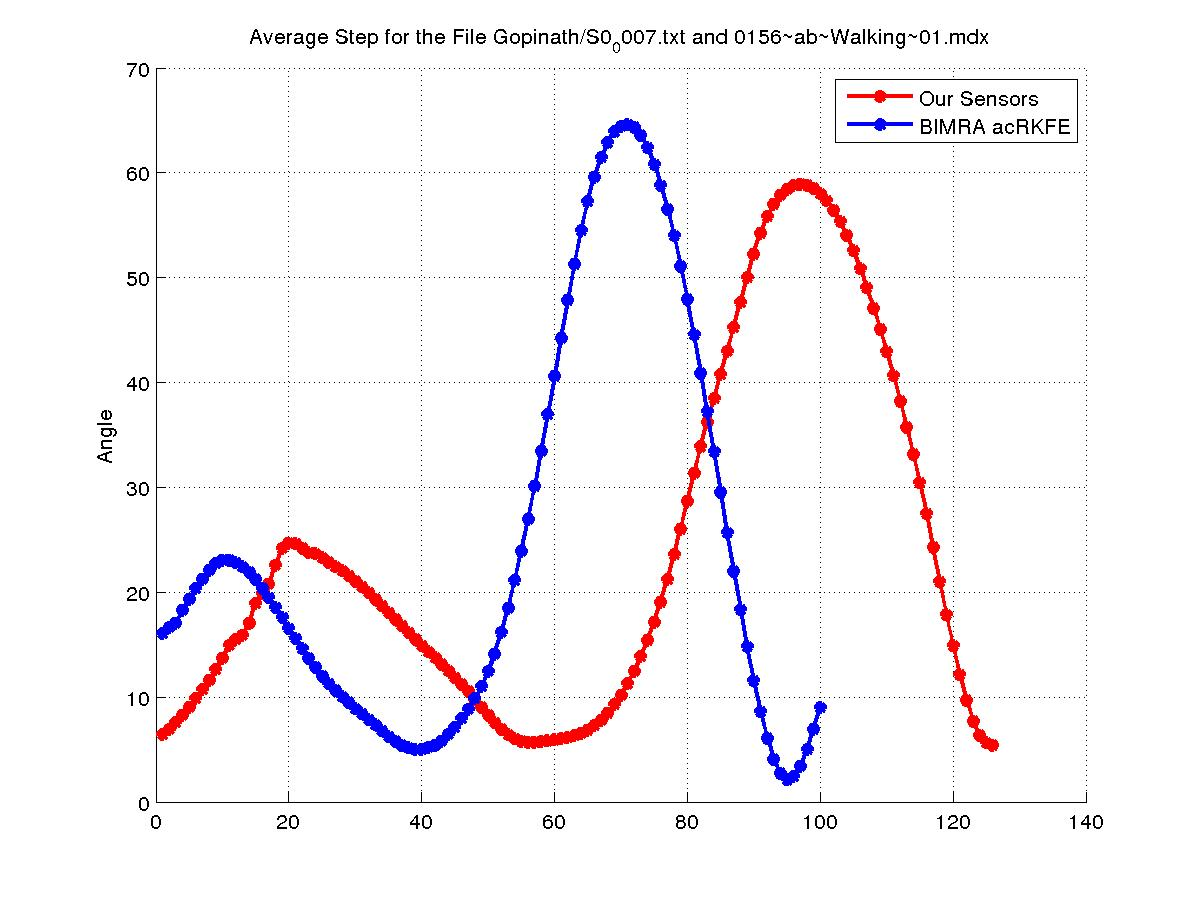
\includegraphics[scale=.22]{S0_0007_before.jpg}
\caption{Before}
\end{subfigure}
\hfill\hfill
\begin{subfigure}[h]{0.4\textwidth}
\hspace*{-2cm} 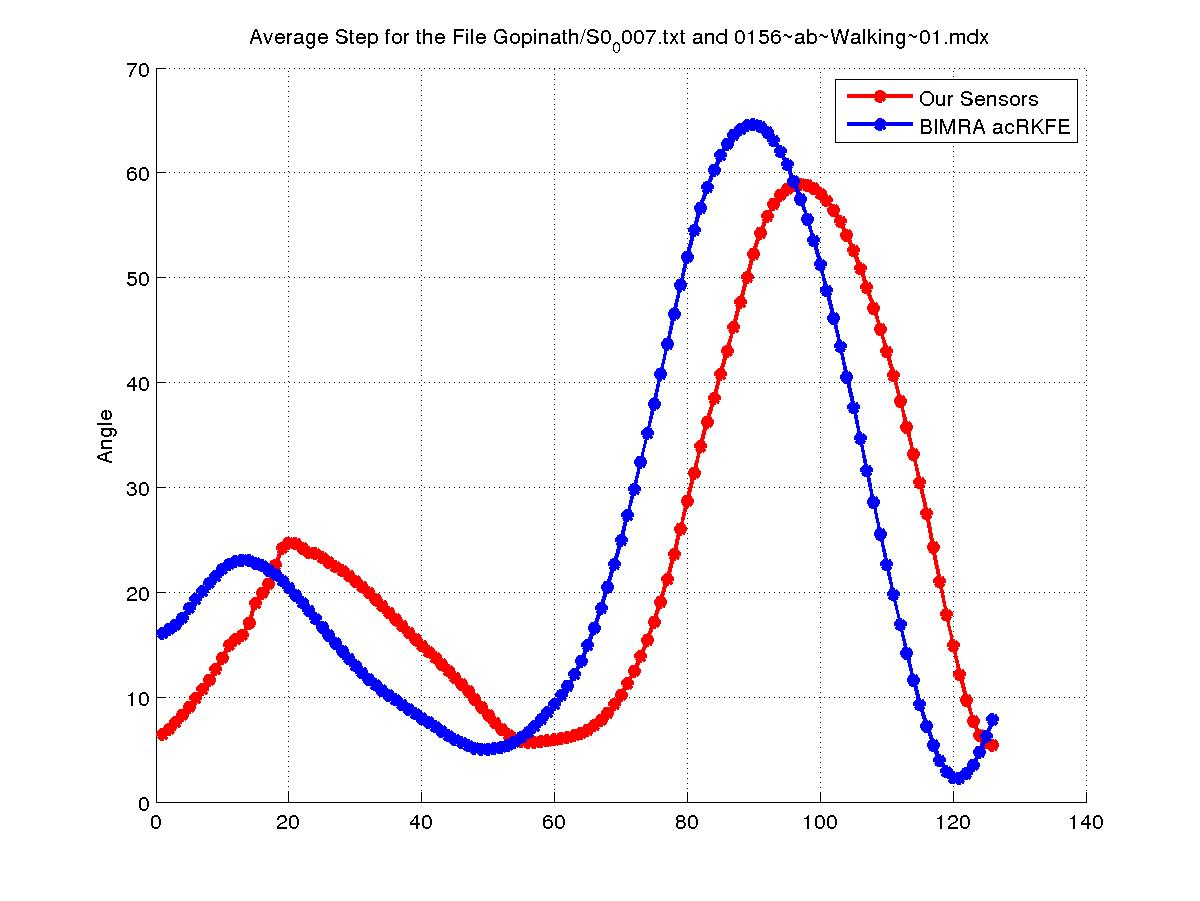
\includegraphics[scale=.22]{S0_0007_after.jpg}
\caption{After}
\end{subfigure}%

\caption[Hello]{Comparison of the Step, Before and After}
\end{figure}

\begin{figure}[h]%

\begin{subfigure}[!htb]{2cm}
\hspace*{-2cm} 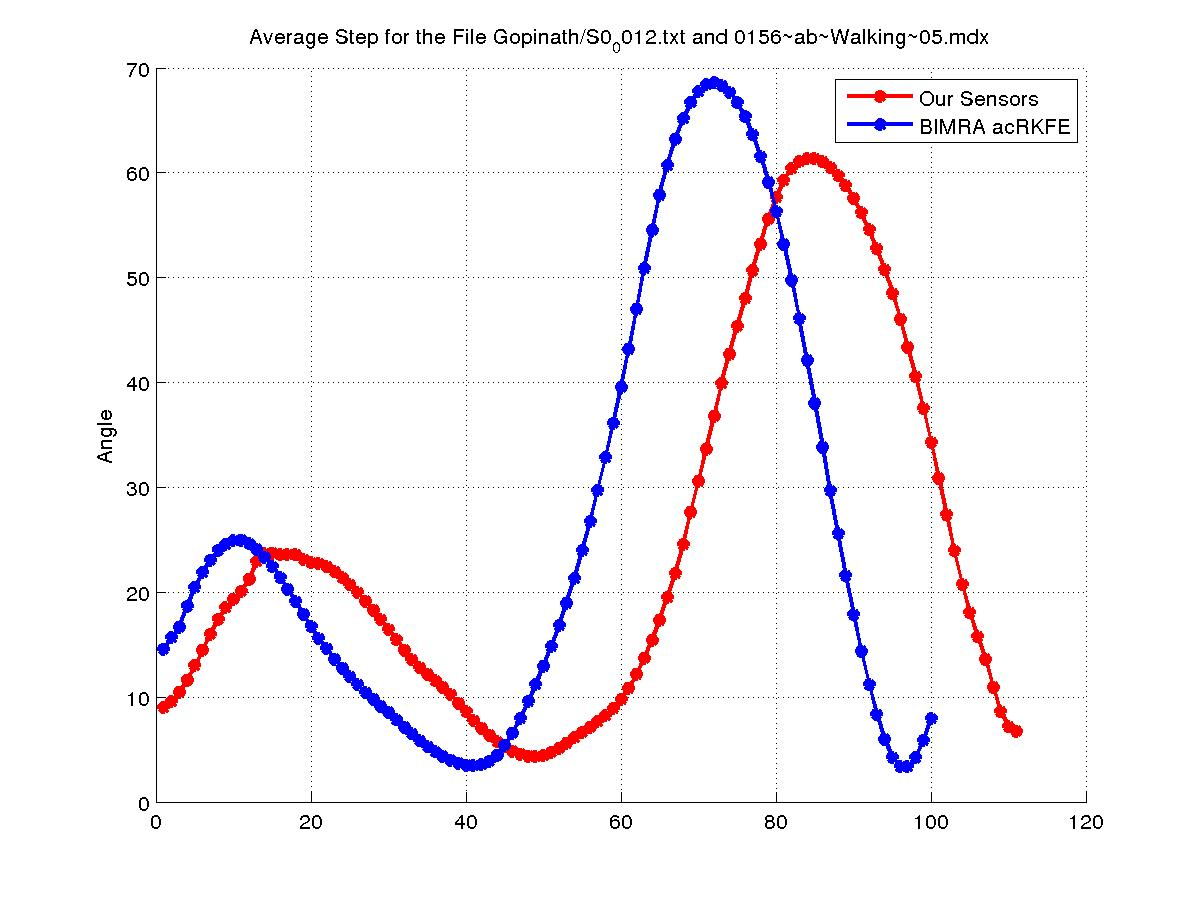
\includegraphics[scale=.22]{S0_0012_before.jpg}
\caption{Before}
\end{subfigure}
\hfill\hfill
\begin{subfigure}[h]{0.4\textwidth}
\hspace*{-2cm} 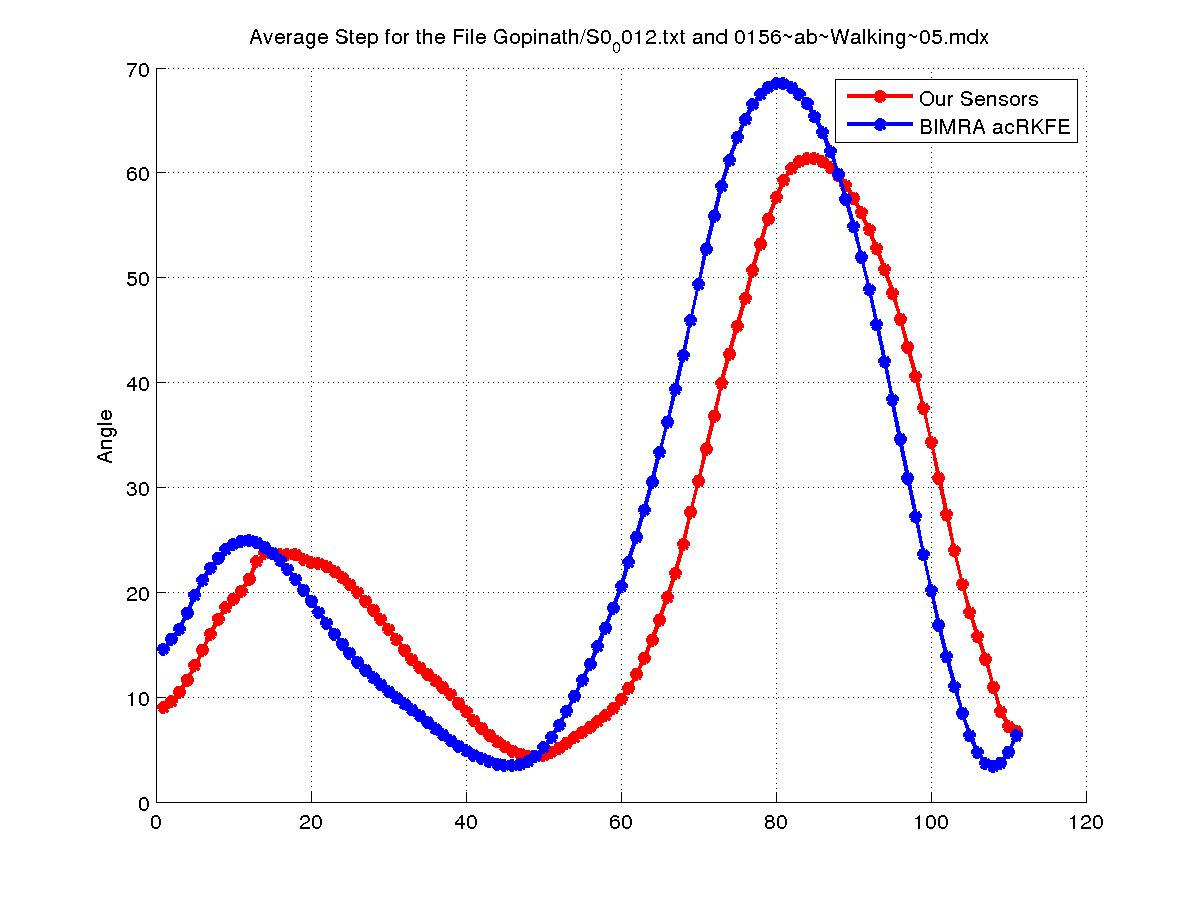
\includegraphics[scale=.22]{S0_0012_after.jpg}
\caption{After}
\end{subfigure}%

\caption[Hello]{Comparison of the Step, Before and After}
\end{figure}

\begin{figure}[h]%

\begin{subfigure}[!htb]{2cm}
\hspace*{-2cm} 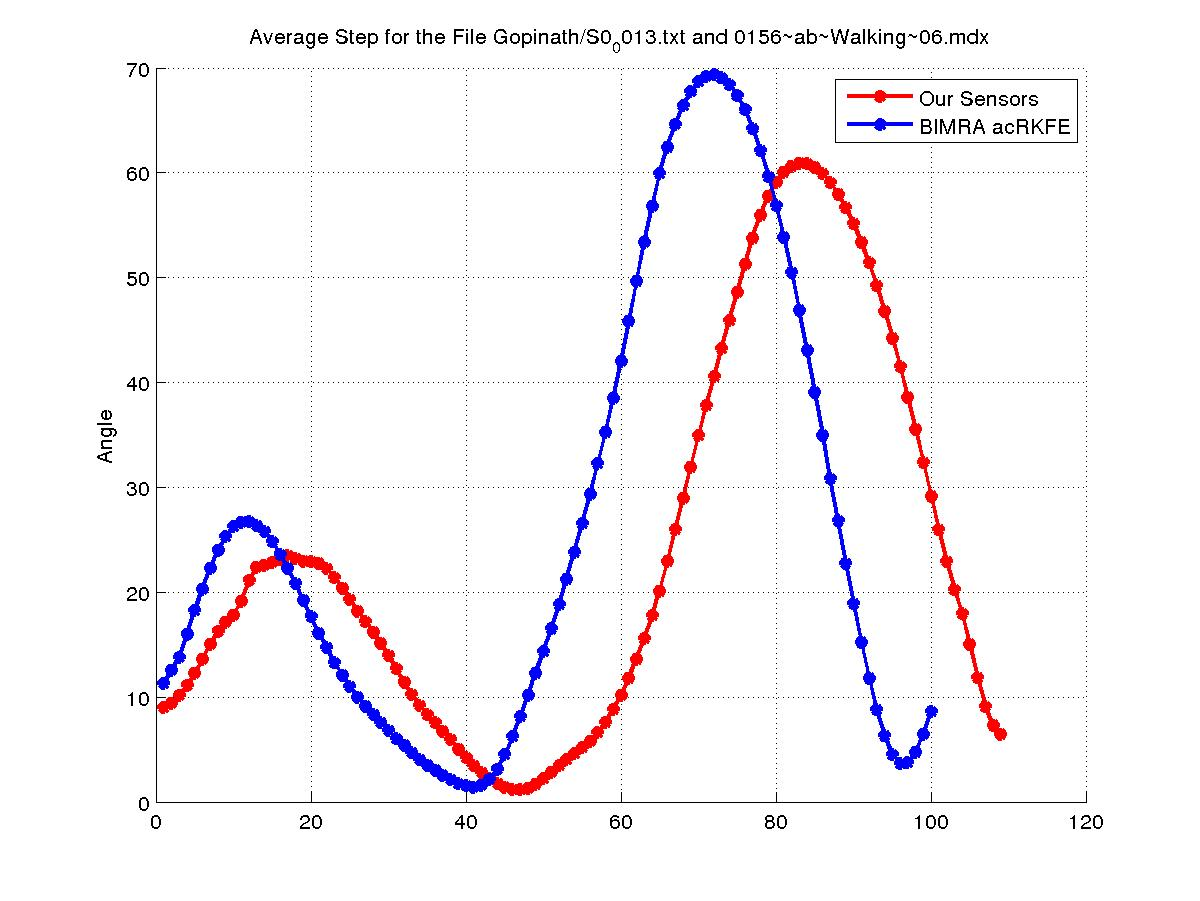
\includegraphics[scale=.22]{S0_0013_before.jpg}
\caption{Before}
\end{subfigure}
\hfill\hfill
\begin{subfigure}[h]{0.4\textwidth}
\hspace*{-2cm} 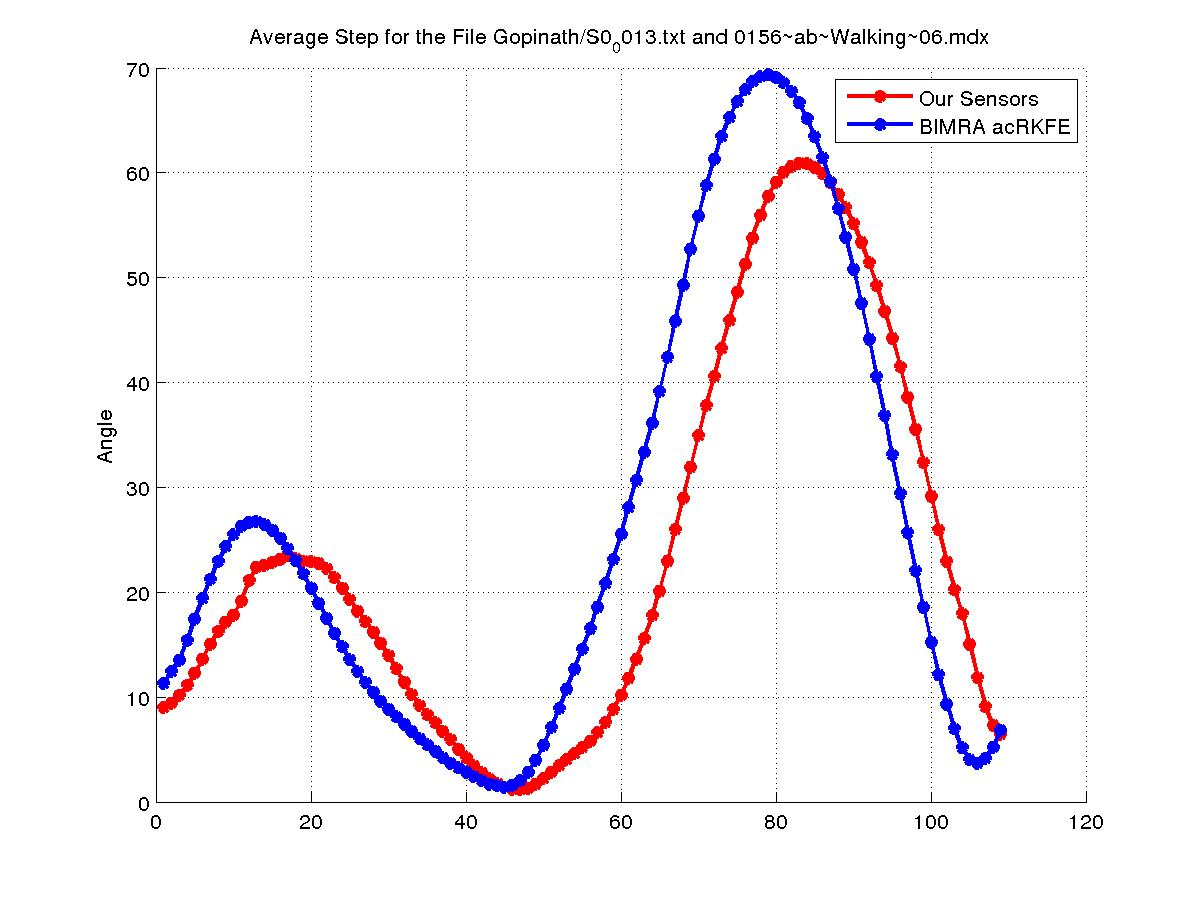
\includegraphics[scale=.22]{S0_0013_after.jpg}
\caption{After}
\end{subfigure}%

\caption[Hello]{Comparison of the Step, Before and After}
\end{figure}

\begin{figure}[h]%

\begin{subfigure}[!htb]{2cm}
\hspace*{-2cm} 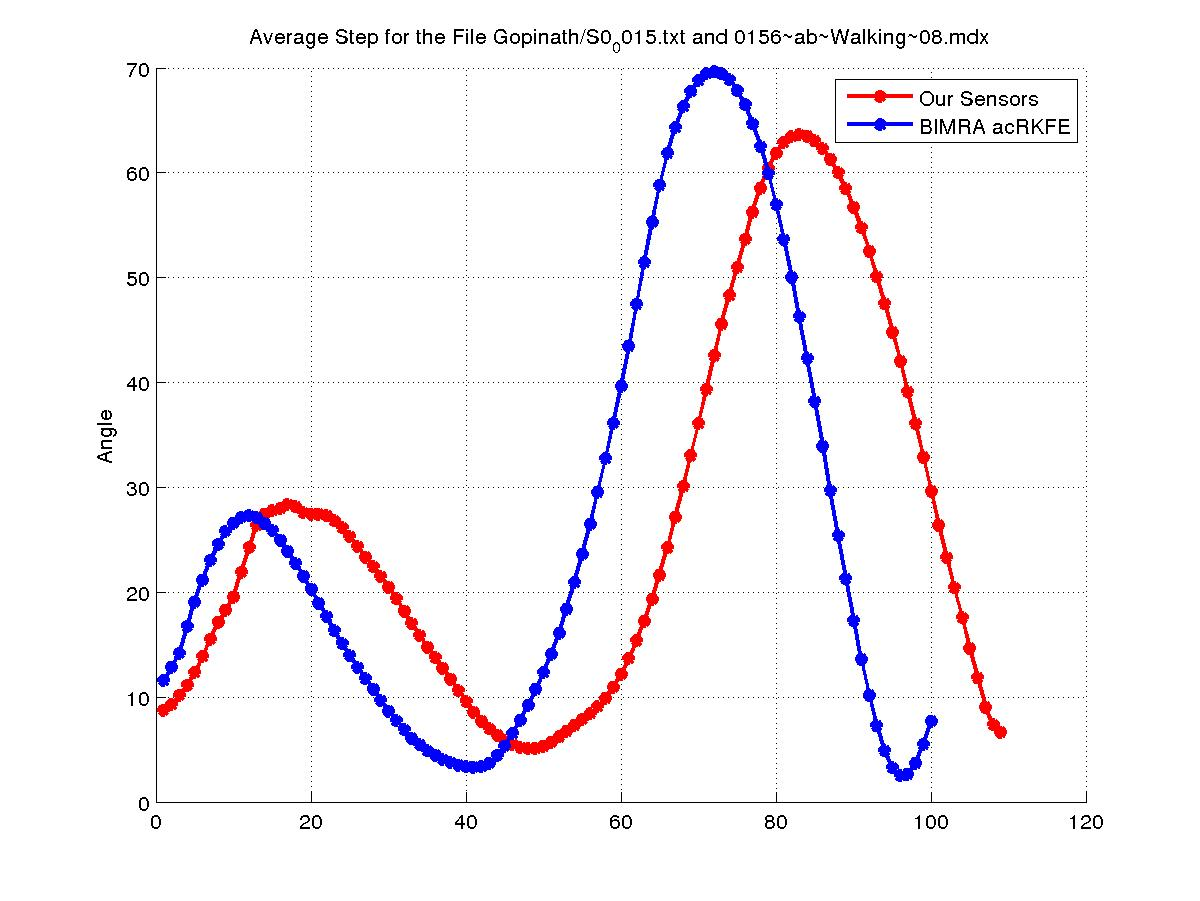
\includegraphics[scale=.22]{S0_0015_before.jpg}
\caption{Before}
\end{subfigure}
\hfill\hfill
\begin{subfigure}[h]{0.4\textwidth}
\hspace*{-2cm} 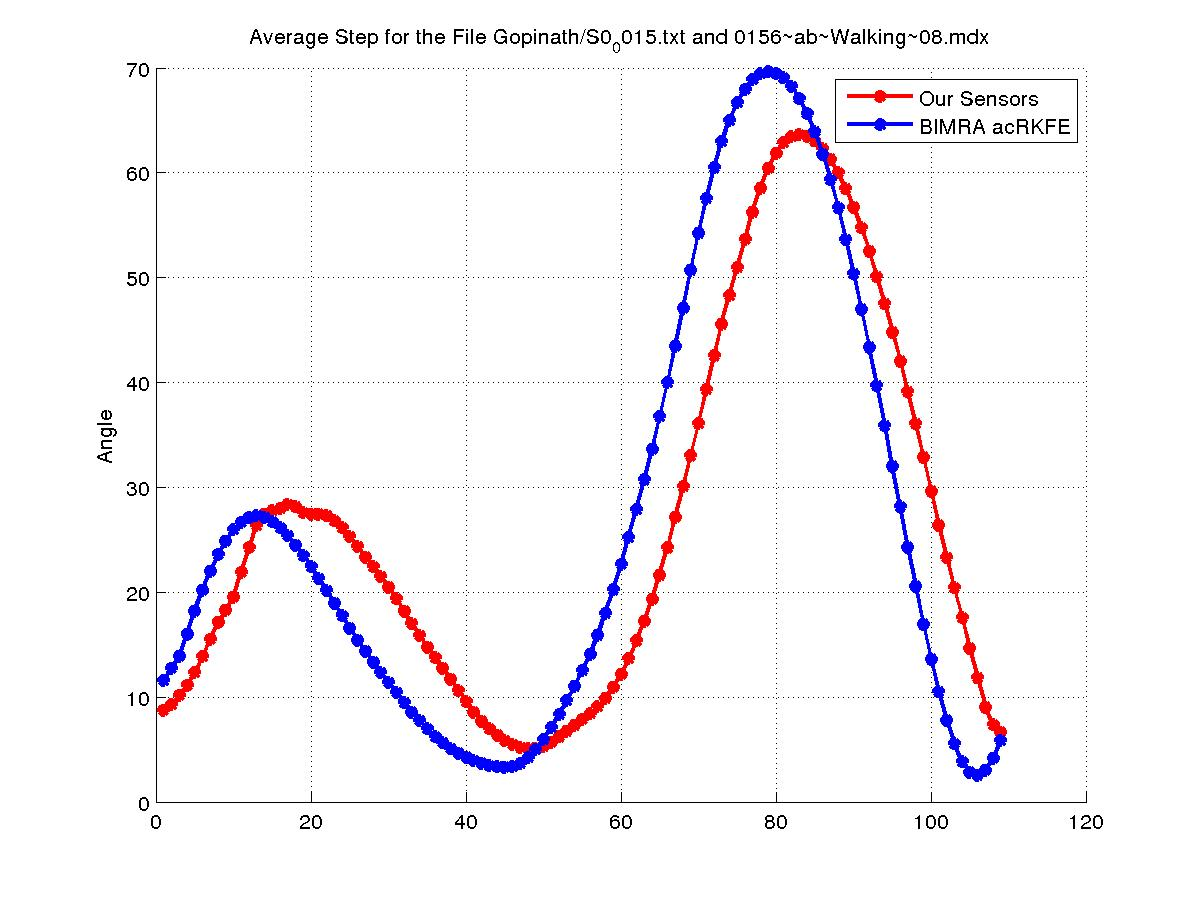
\includegraphics[scale=.22]{S0_0015_after.jpg}
\caption{After}
\end{subfigure}%

\caption[Hello]{Comparison of the Step, Before and After}
\end{figure}

\begin{figure}[h]%

\begin{subfigure}[!htb]{2cm}
\hspace*{-2cm} 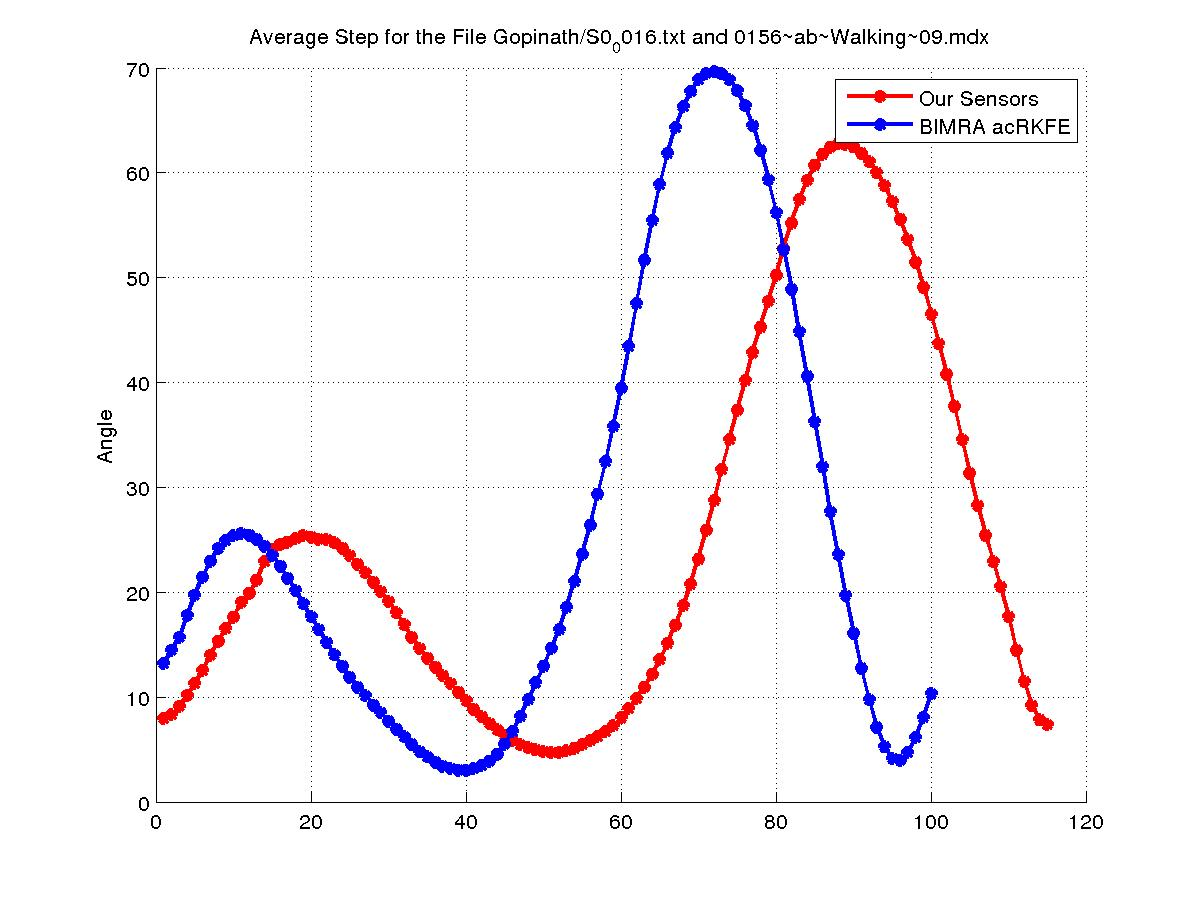
\includegraphics[scale=.22]{S0_0016_before.jpg}
\caption{Before}
\end{subfigure}
\hfill\hfill
\begin{subfigure}[h]{0.4\textwidth}
\hspace*{-2cm} 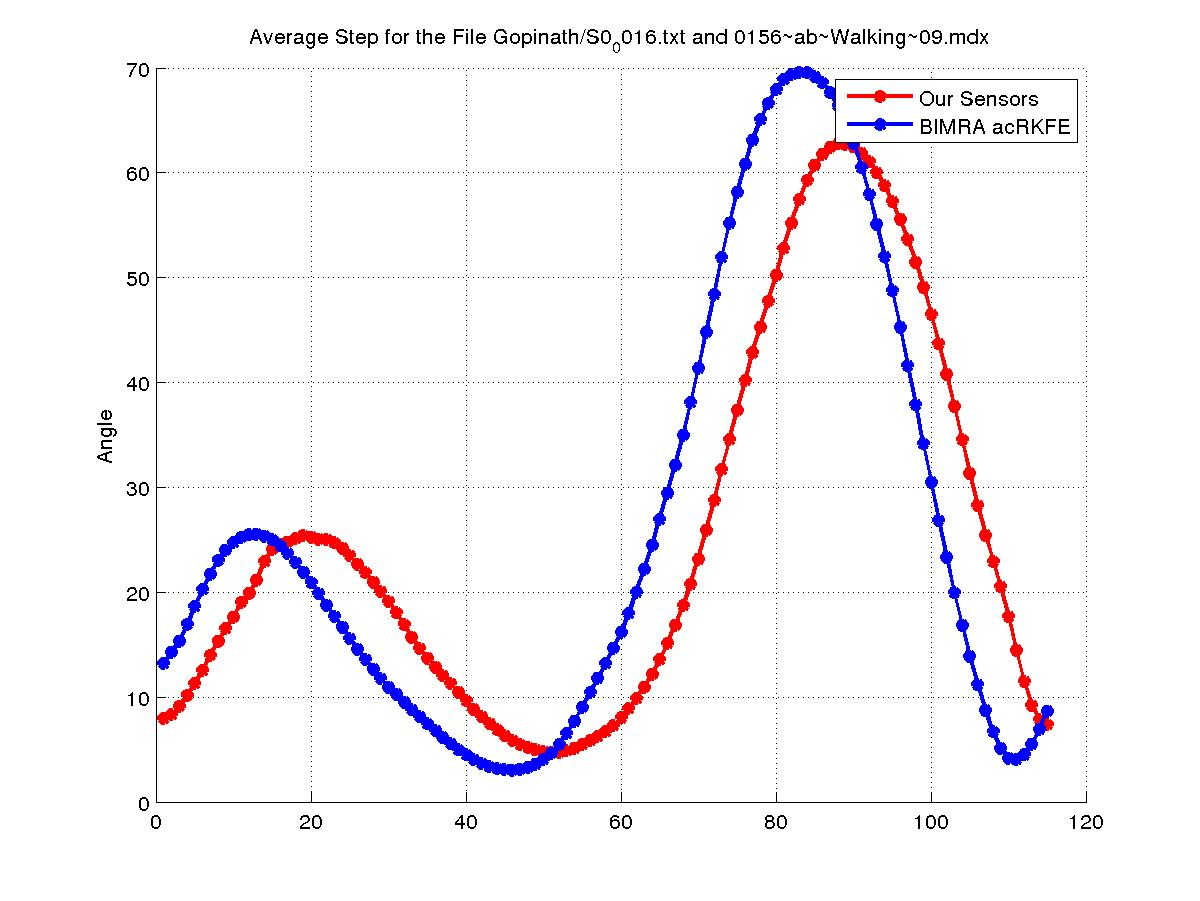
\includegraphics[scale=.22]{S0_0016_after.jpg}
\caption{After}
\end{subfigure}%

\caption[Hello]{Comparison of the Step, Before and After}
\end{figure}

\begin{figure}[h]%

\begin{subfigure}[!htb]{2cm}
\hspace*{-2cm} 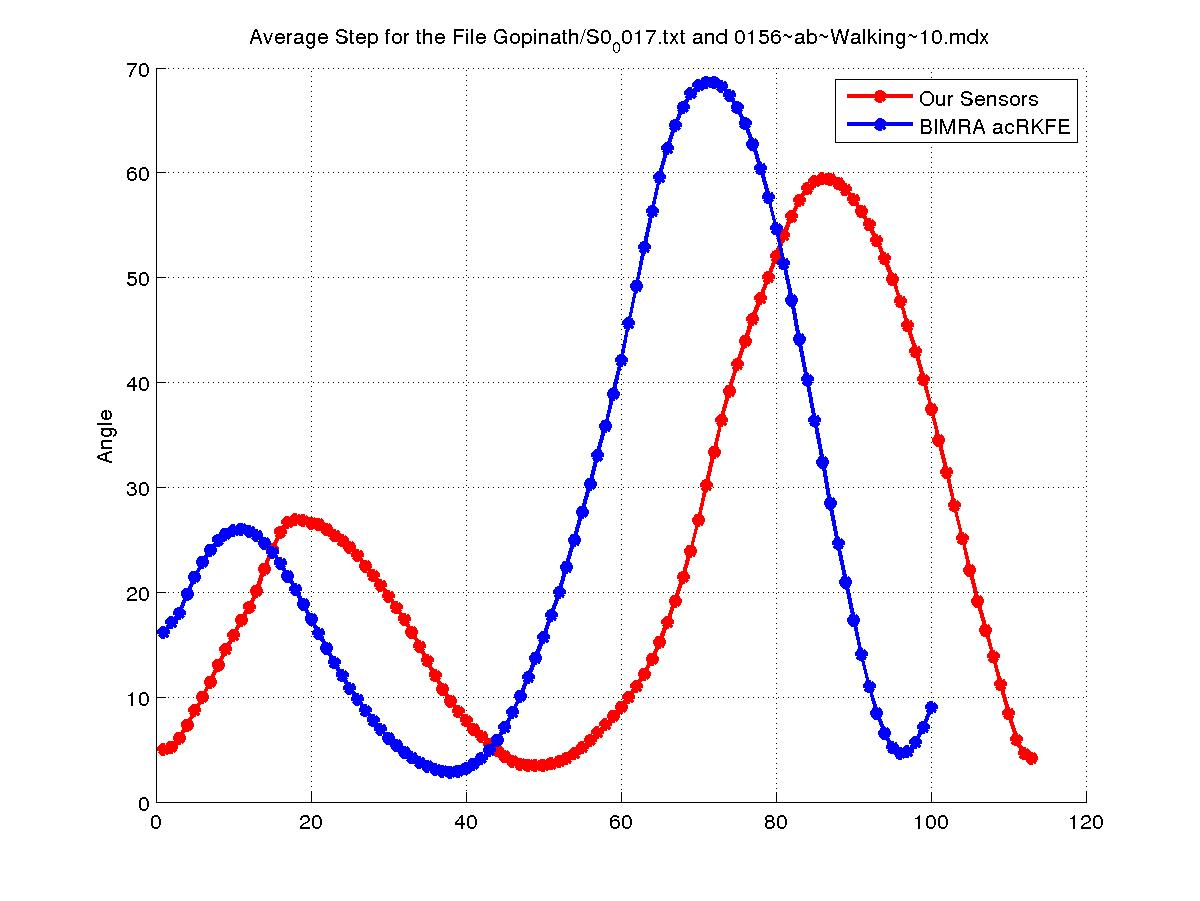
\includegraphics[scale=.22]{S0_0017_before.jpg}
\caption{Before}
\end{subfigure}
\hfill\hfill
\begin{subfigure}[h]{0.4\textwidth}
\hspace*{-2cm} 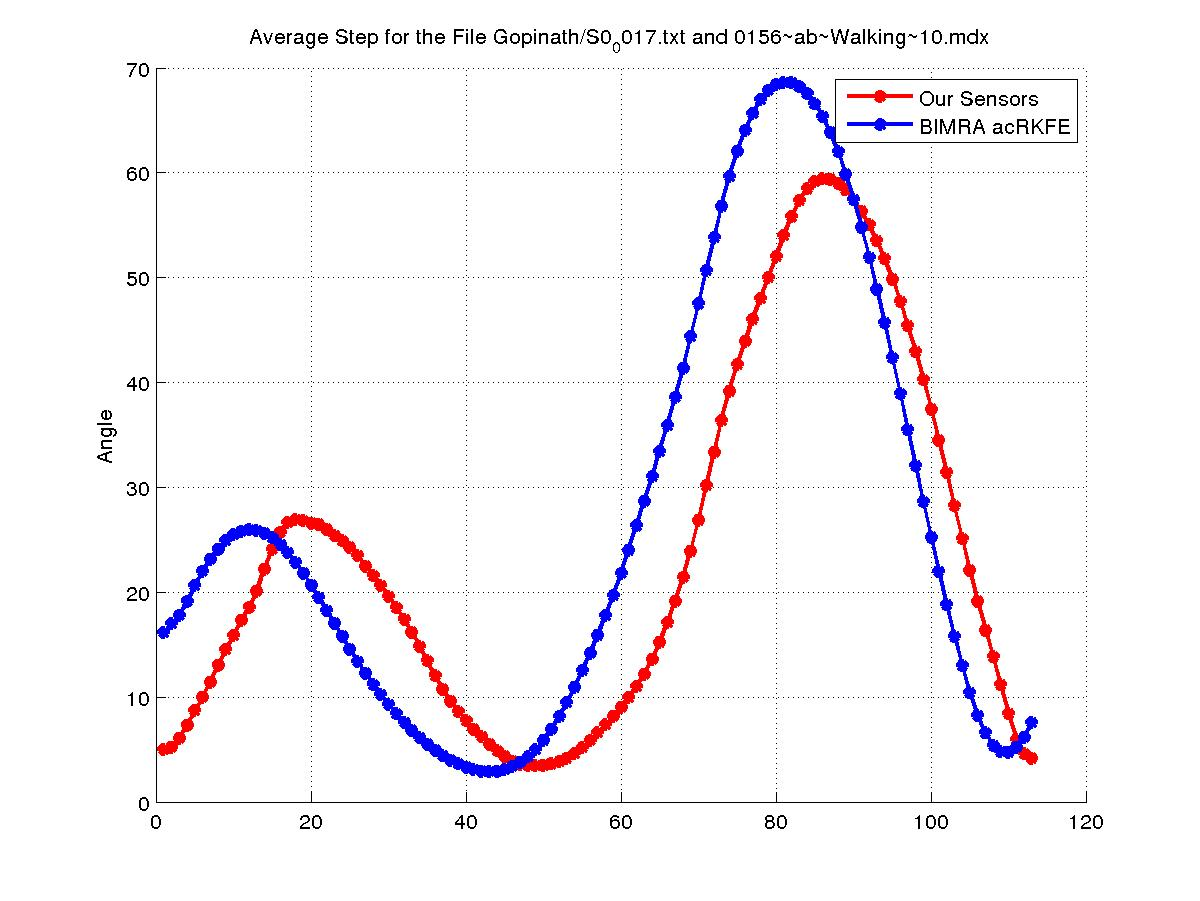
\includegraphics[scale=.22]{S0_0017_after.jpg}
\caption{After}
\end{subfigure}%

\caption[Hello]{Comparison of the Step, Before and After}
\end{figure}

\FloatBarrier

\subsection*{Comparison of Rest of the Steps, using acmRKFE}
\begin{figure}[h]%

\begin{subfigure}[!htb]{2cm}
\hspace*{-2cm} 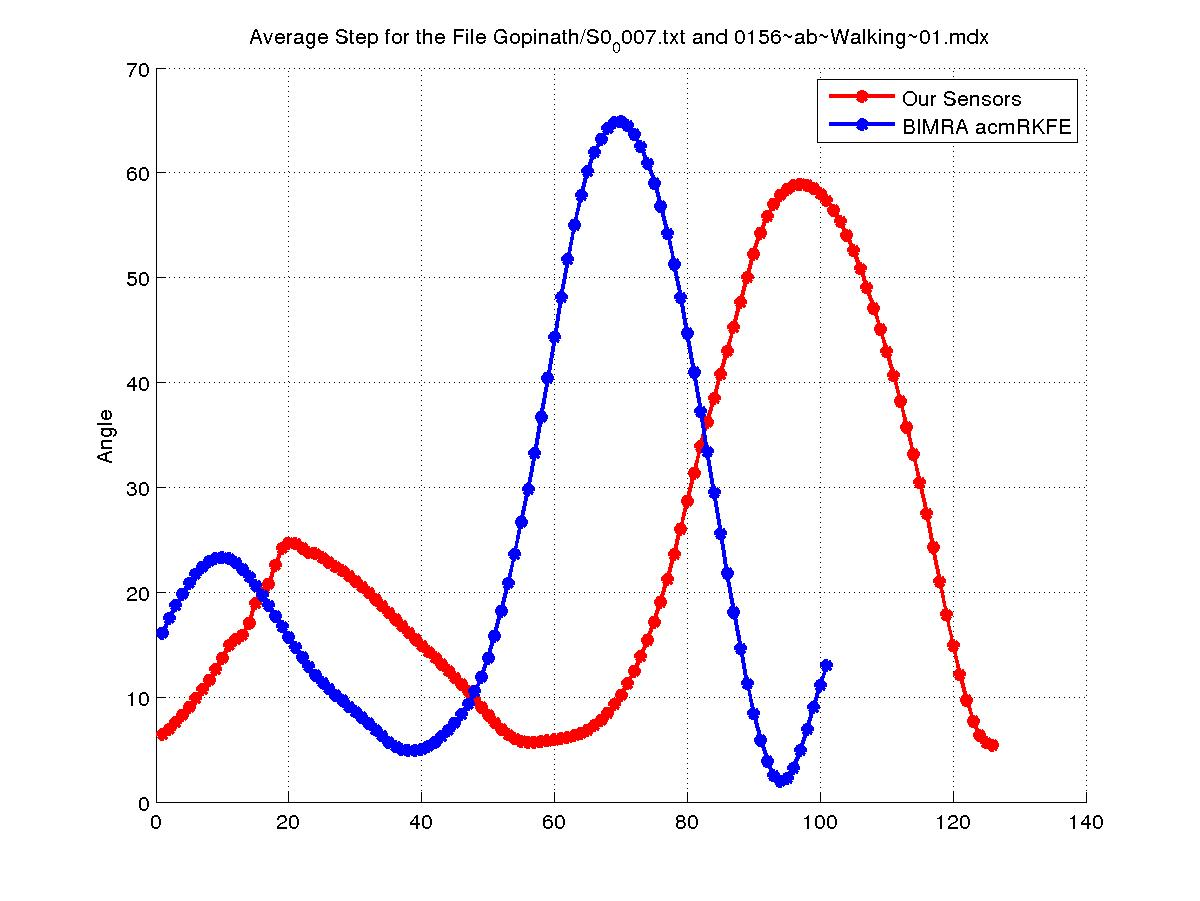
\includegraphics[scale=.22]{S0_0007_before_acmrkfe.jpg}
\caption{Before}
\end{subfigure}
\hfill\hfill
\begin{subfigure}[h]{0.4\textwidth}
\hspace*{-2cm} 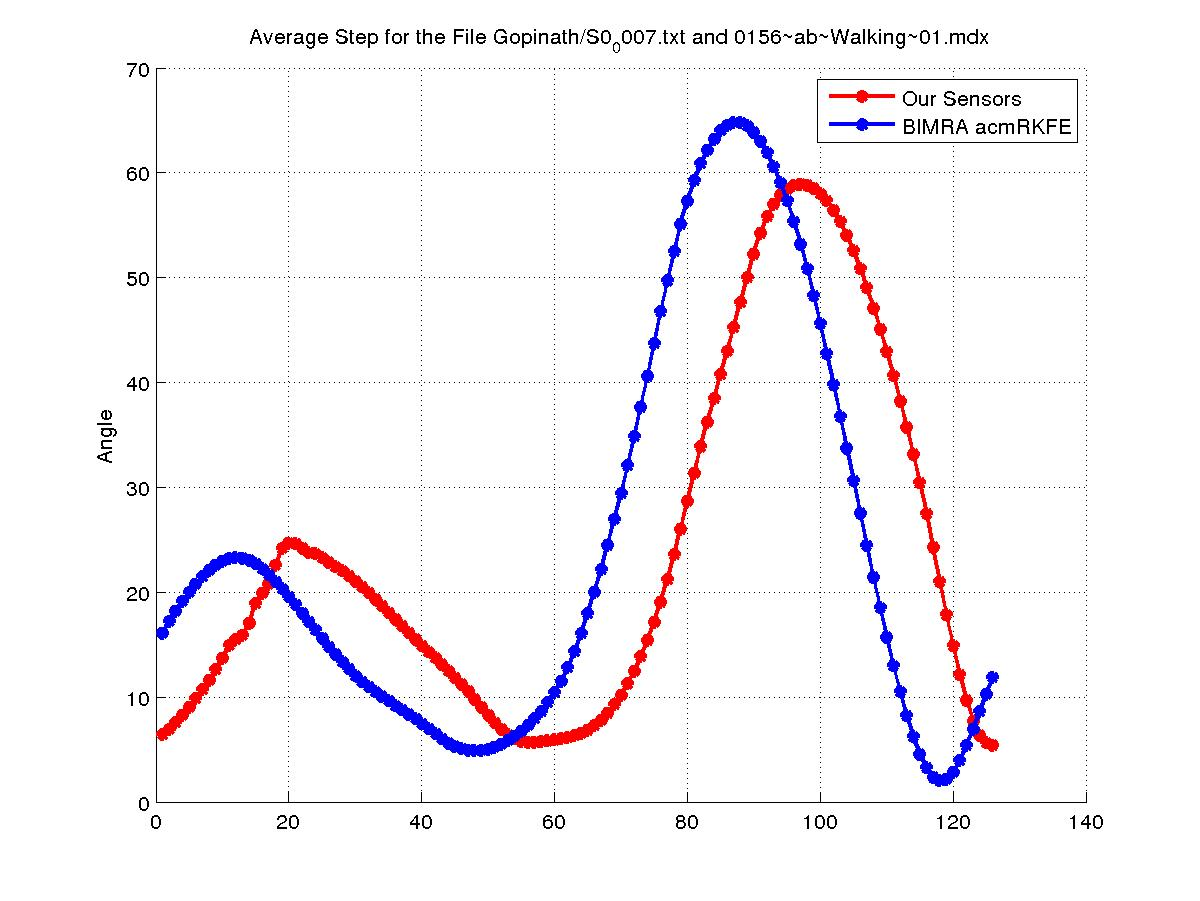
\includegraphics[scale=.22]{S0_0007_after_acmrkfe.jpg}
\caption{After}
\end{subfigure}%

\caption[Hello]{Comparison of the Step, Before and After}
\end{figure}

\begin{figure}[h]%

\begin{subfigure}[!htb]{2cm}
\hspace*{-2cm} 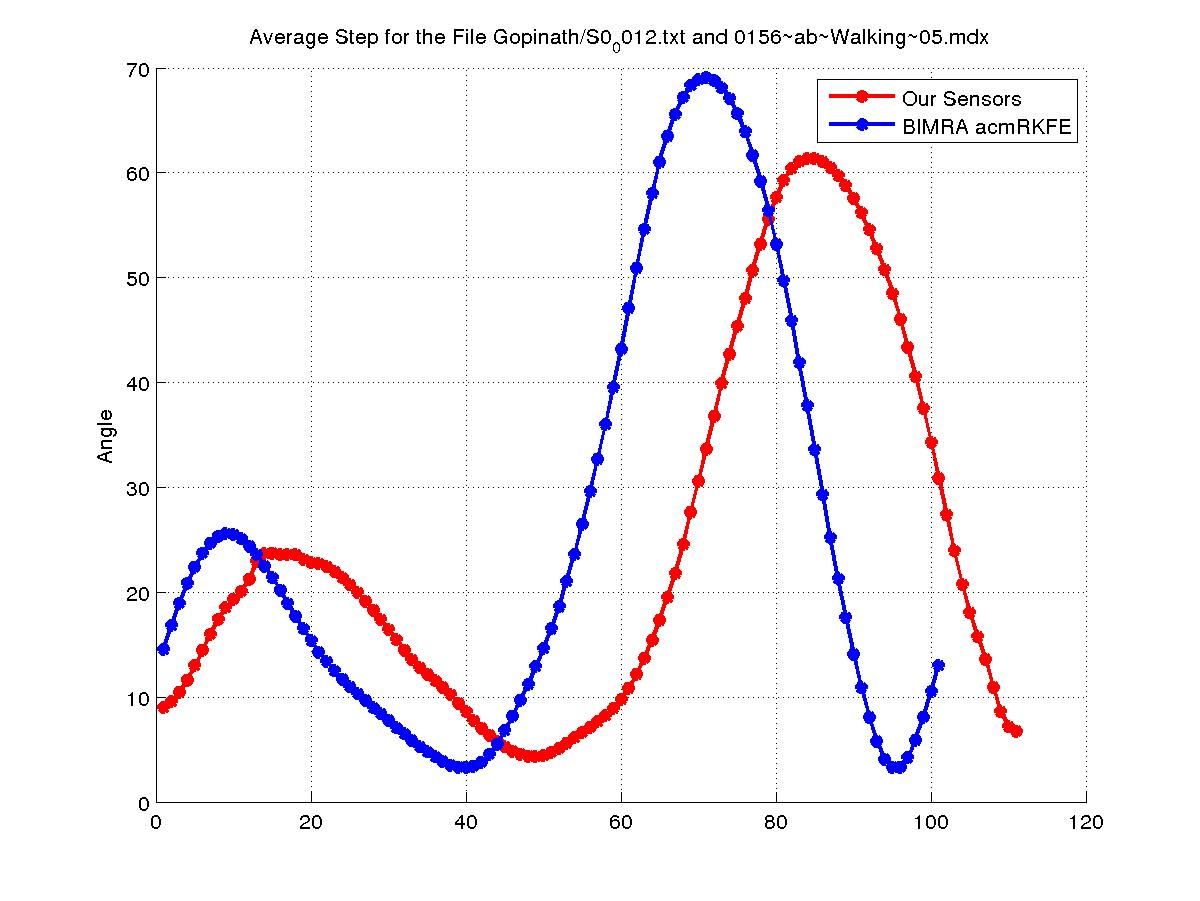
\includegraphics[scale=.22]{S0_0012_before_acmrkfe.jpg}
\caption{Before}
\end{subfigure}
\hfill\hfill
\begin{subfigure}[h]{0.4\textwidth}
\hspace*{-2cm} 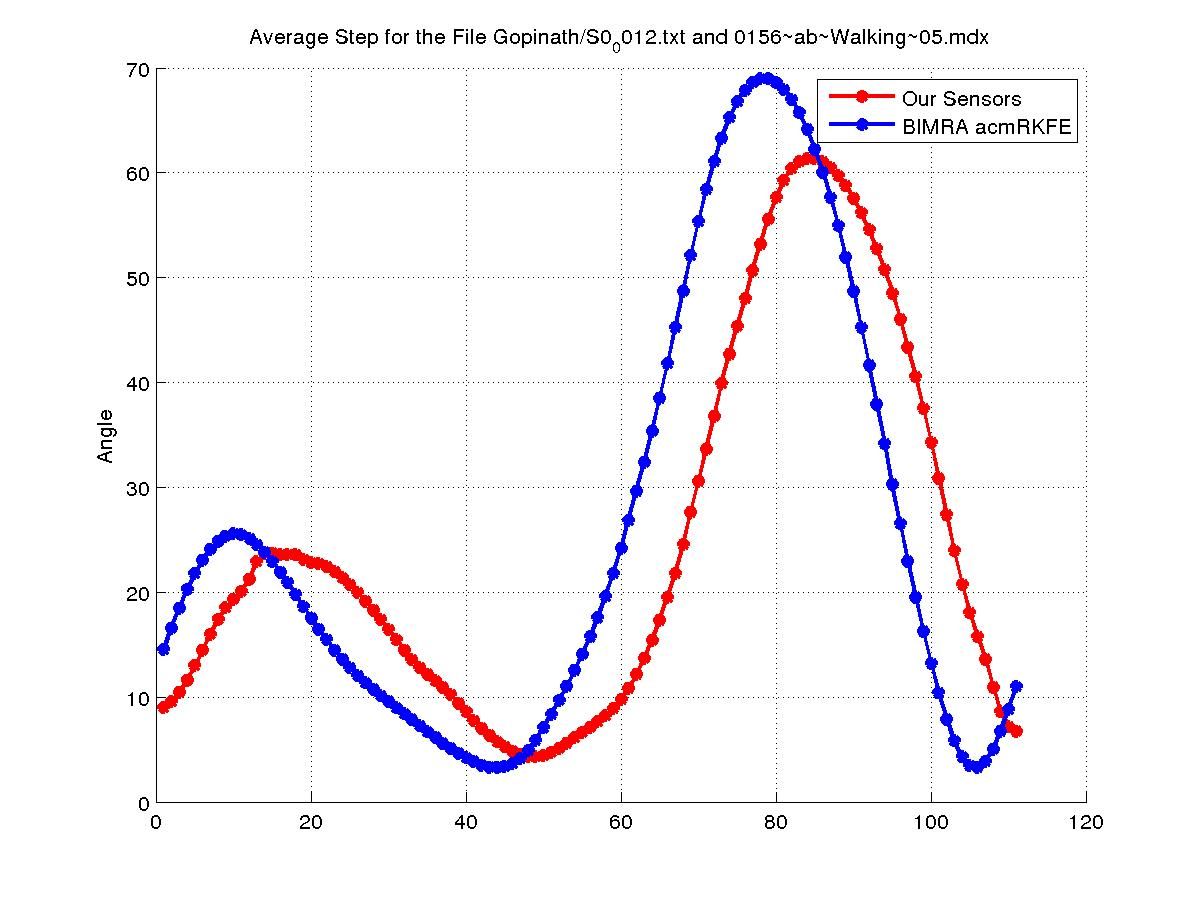
\includegraphics[scale=.22]{S0_0012_after_acmrkfe.jpg}
\caption{After}
\end{subfigure}%

\caption[Hello]{Comparison of the Step, Before and After}
\end{figure}

\begin{figure}[h]%

\begin{subfigure}[!htb]{2cm}
\hspace*{-2cm} 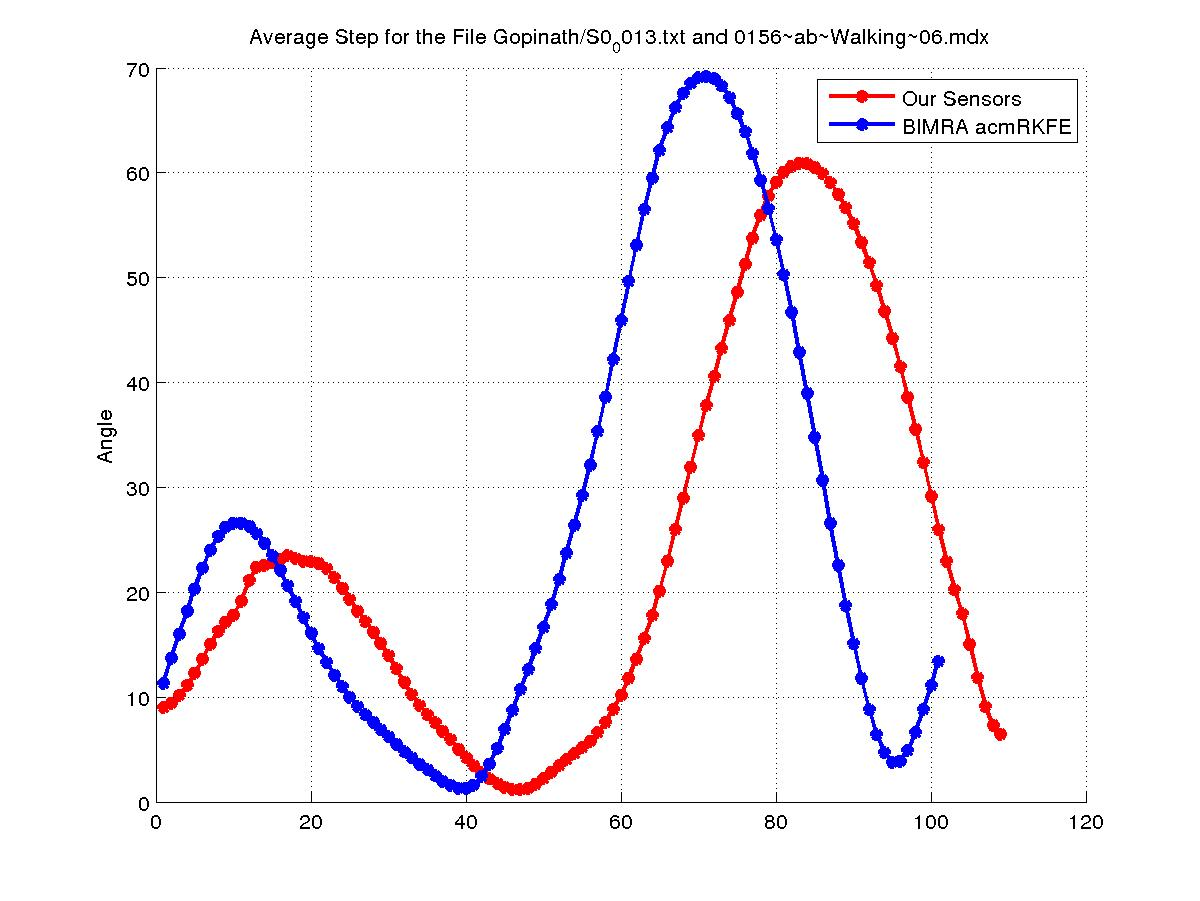
\includegraphics[scale=.22]{S0_0013_before_acmrkfe.jpg}
\caption{Before}
\end{subfigure}
\hfill\hfill
\begin{subfigure}[h]{0.4\textwidth}
\hspace*{-2cm} 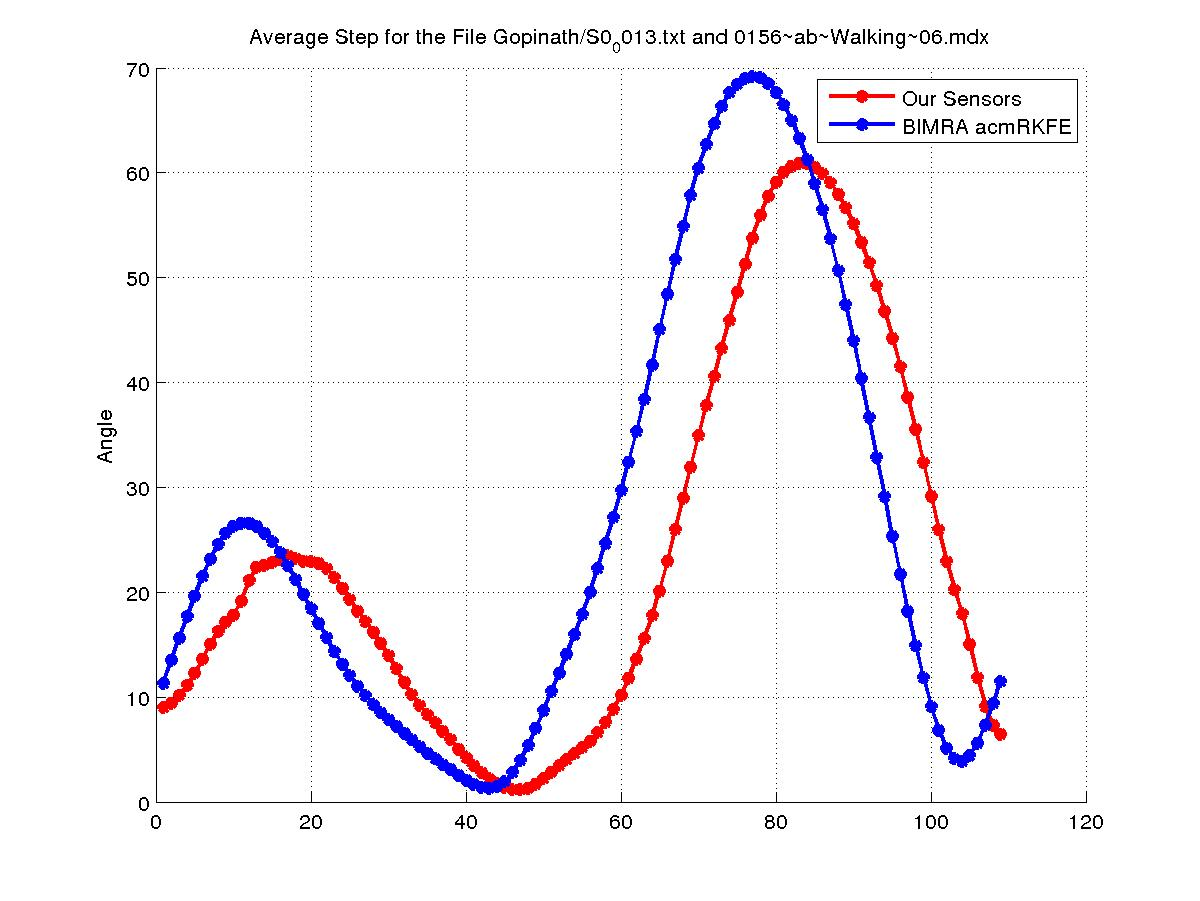
\includegraphics[scale=.22]{S0_0013_after_acmrkfe.jpg}
\caption{After}
\end{subfigure}%

\caption[Hello]{Comparison of the Step, Before and After}
\end{figure}

\begin{figure}[h]%

\begin{subfigure}[!htb]{2cm}
\hspace*{-2cm} 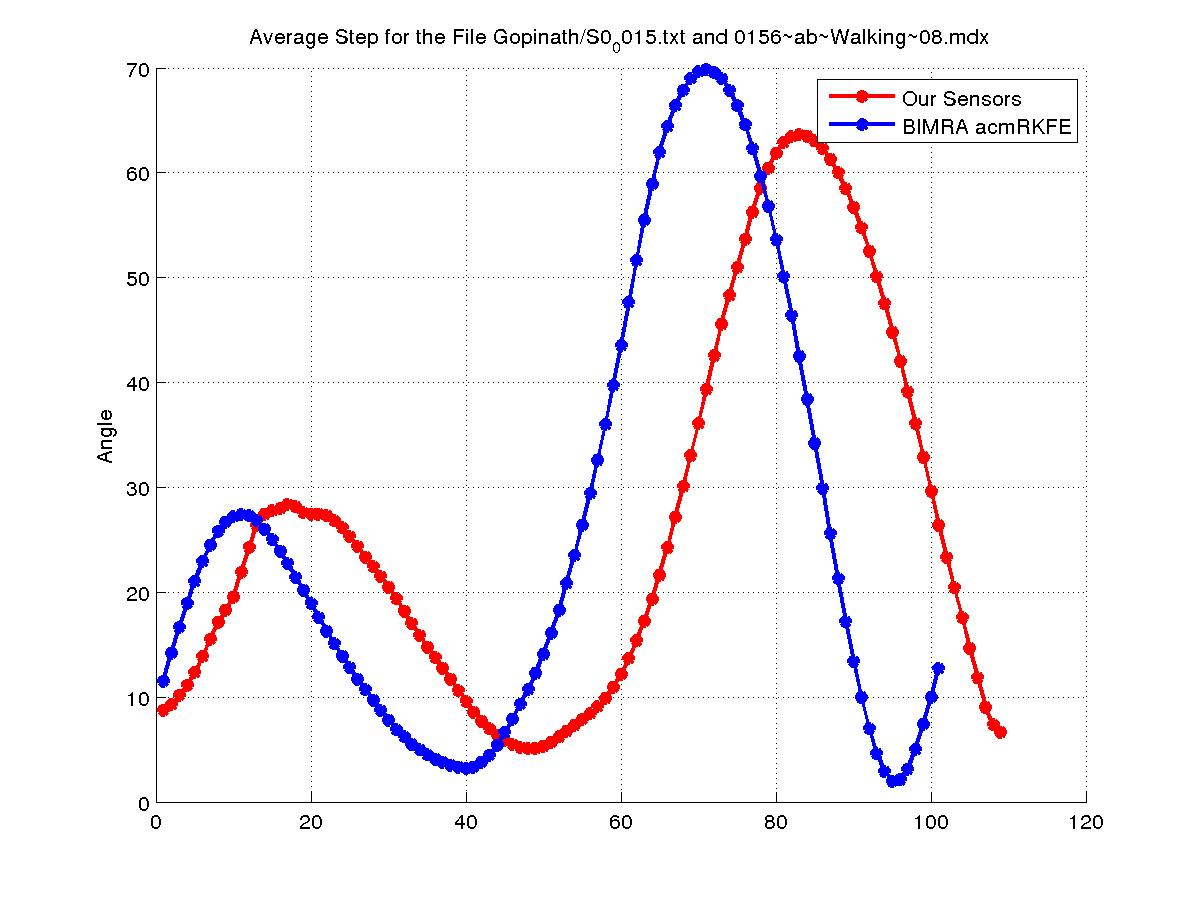
\includegraphics[scale=.22]{S0_0015_before_acmrkfe.jpg}
\caption{Before}
\end{subfigure}
\hfill\hfill
\begin{subfigure}[h]{0.4\textwidth}
\hspace*{-2cm} 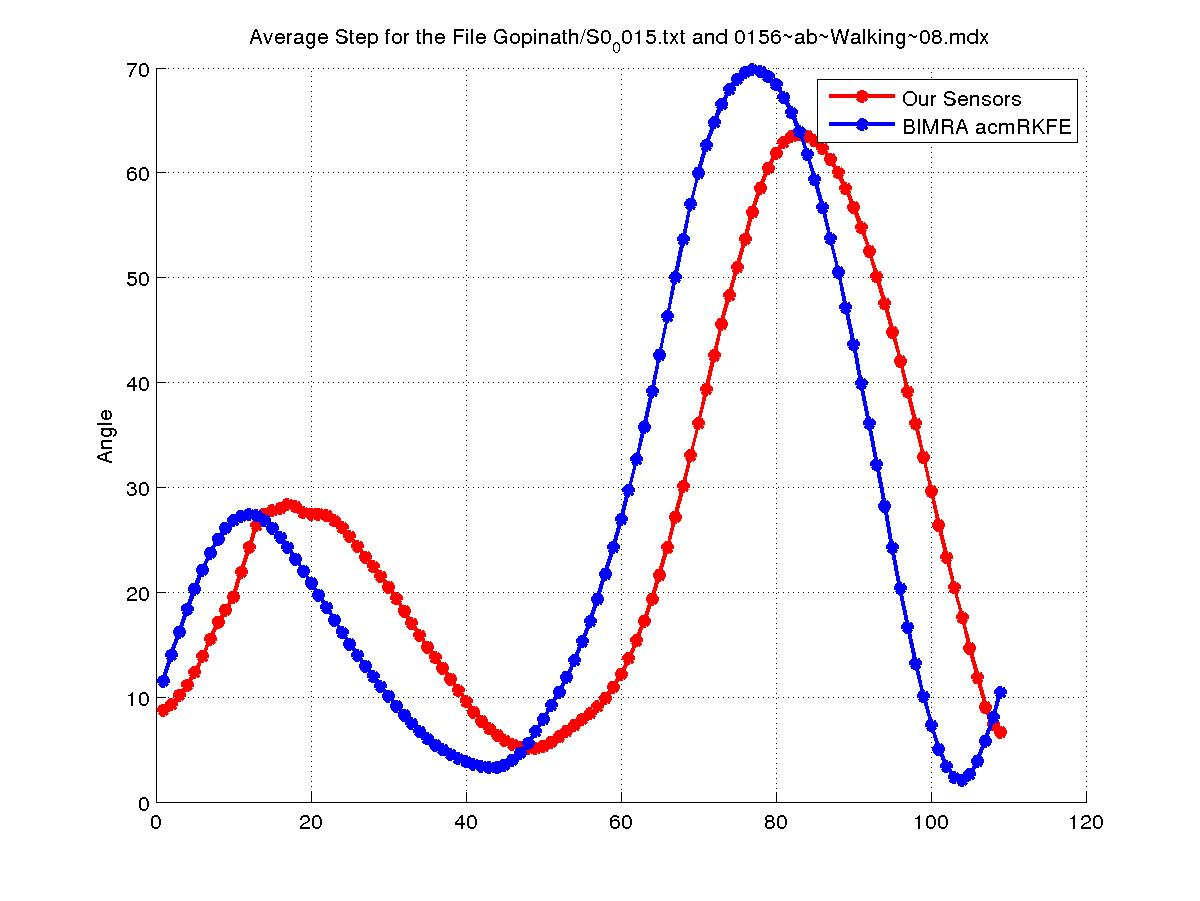
\includegraphics[scale=.22]{S0_0015_after_acmrkfe.jpg}
\caption{After}
\end{subfigure}%

\caption[Hello]{Comparison of the Step, Before and After}
\end{figure}

\begin{figure}[h]%

\begin{subfigure}[!htb]{2cm}
\hspace*{-2cm} 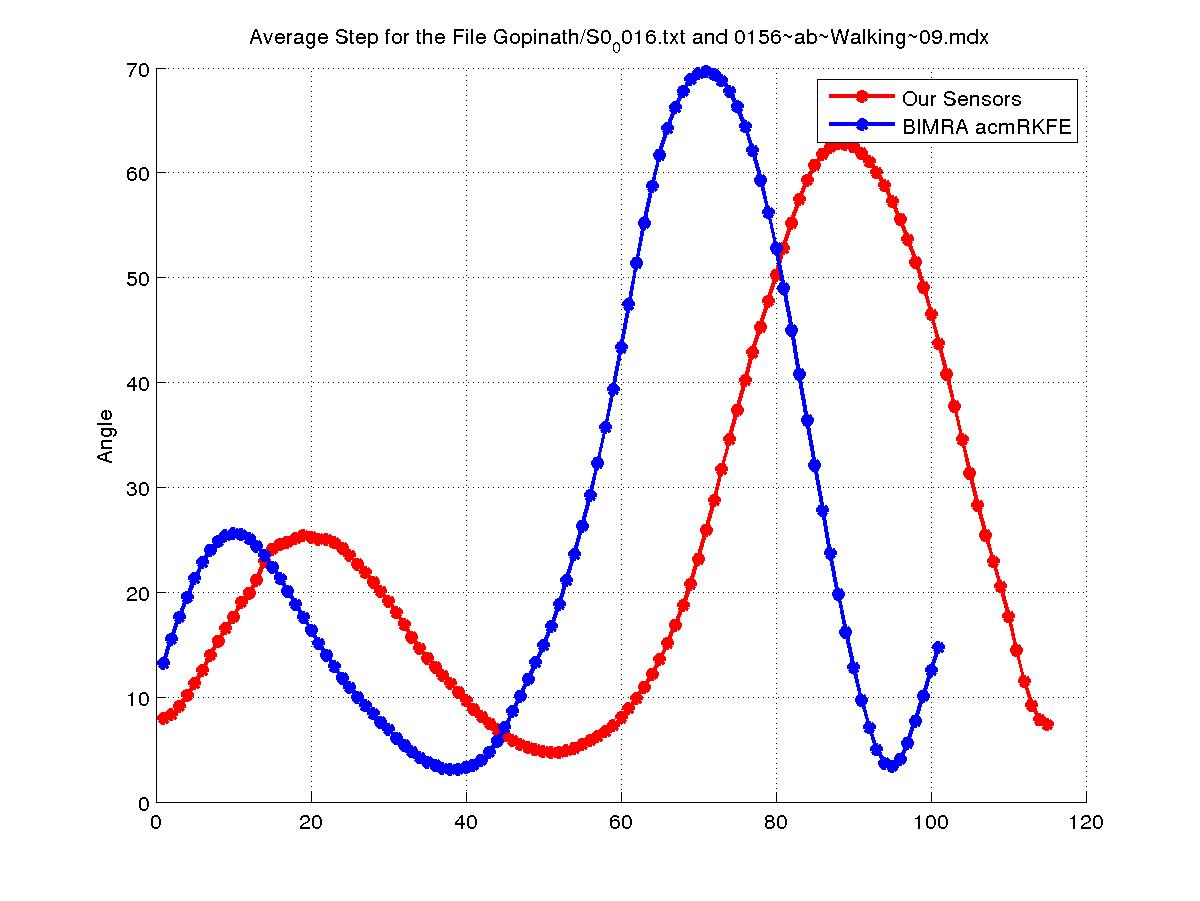
\includegraphics[scale=.22]{S0_0016_before_acmrkfe.jpg}
\caption{Before}
\end{subfigure}
\hfill\hfill
\begin{subfigure}[h]{0.4\textwidth}
\hspace*{-2cm} 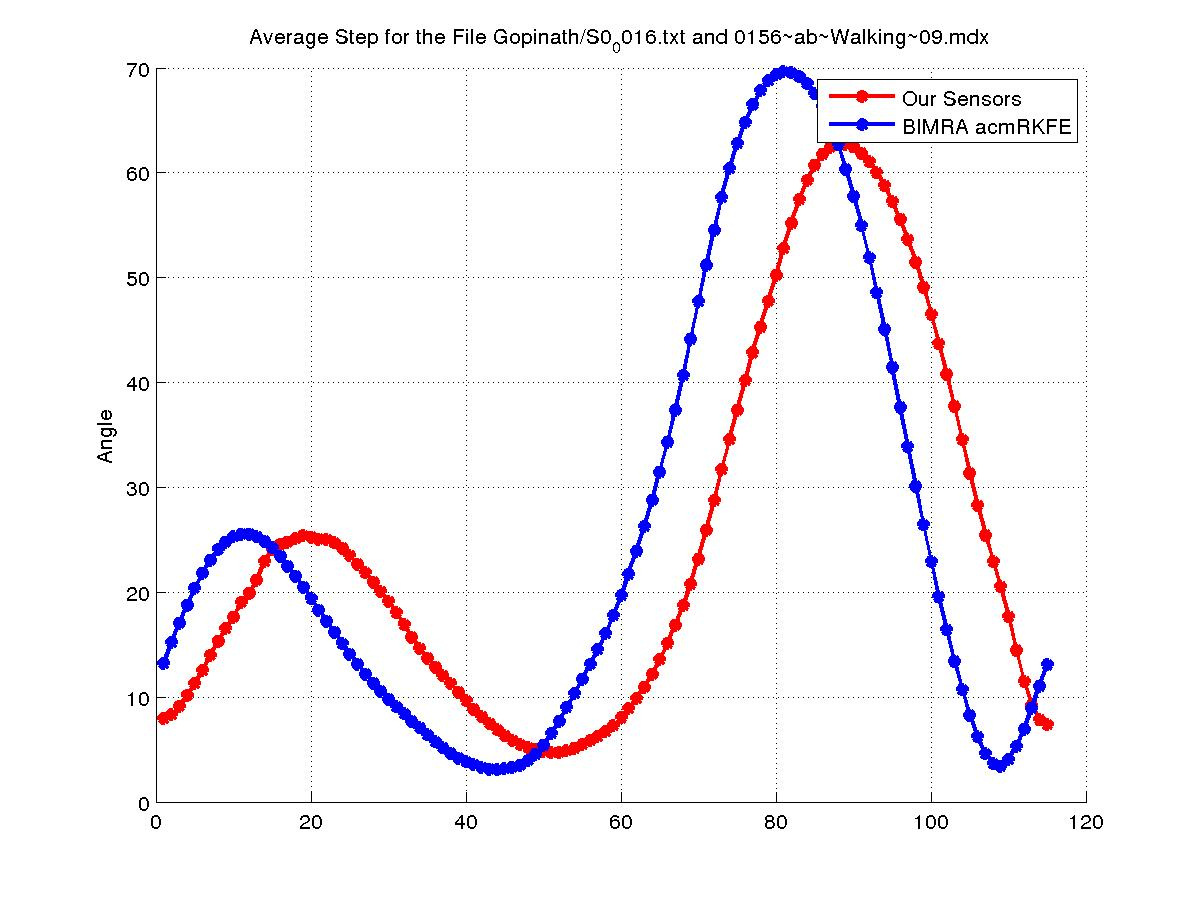
\includegraphics[scale=.22]{S0_0016_after_acmrkfe.jpg}
\caption{After}
\end{subfigure}%

\caption[Hello]{Comparison of the Step, Before and After}
\end{figure}

\begin{figure}[h]%

\begin{subfigure}[!htb]{2cm}
\hspace*{-2cm} 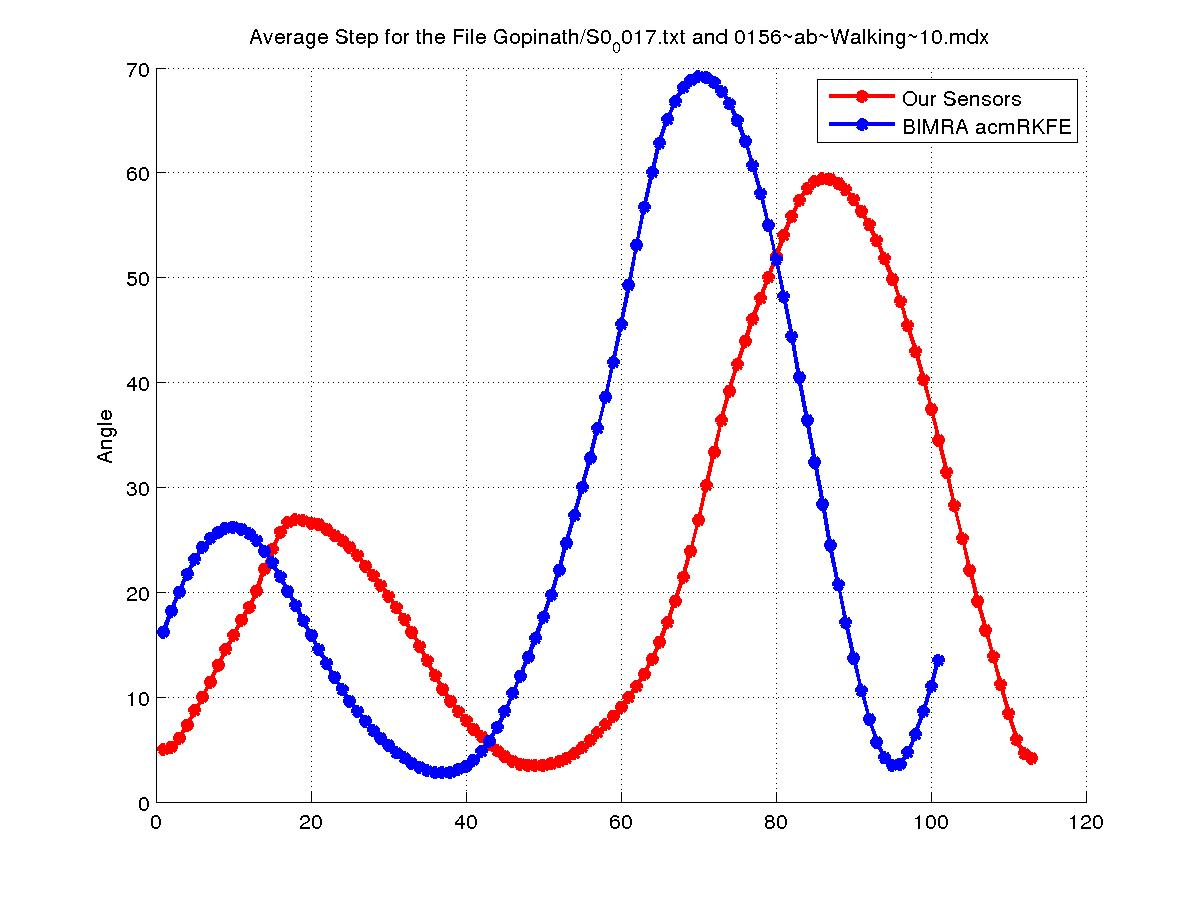
\includegraphics[scale=.22]{S0_0017_before_acmrkfe.jpg}
\caption{Before}
\end{subfigure}
\hfill\hfill
\begin{subfigure}[h]{0.4\textwidth}
\hspace*{-2cm} 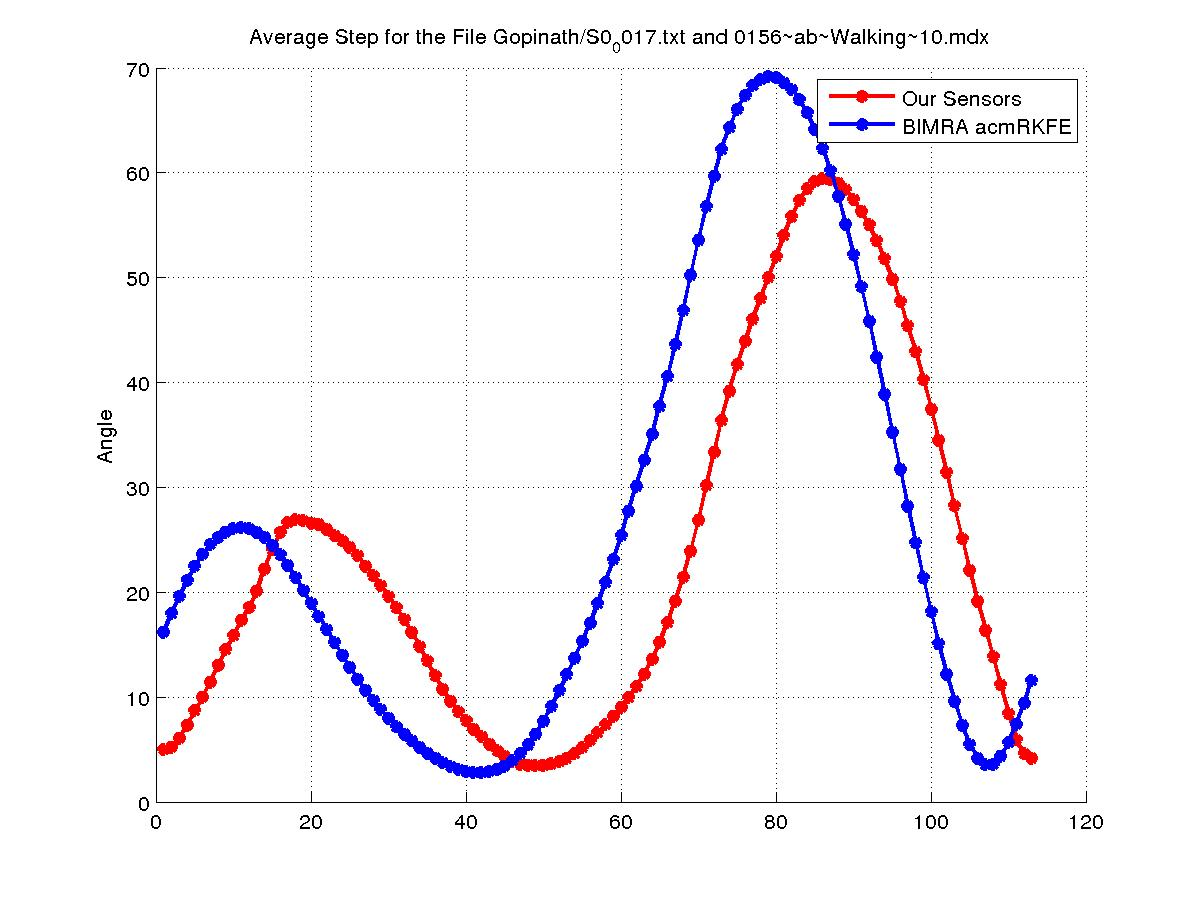
\includegraphics[scale=.22]{S0_0017_after_acmrkfe.jpg}
\caption{After}
\end{subfigure}%

\caption[Hello]{Comparison of the Step, Before and After}
\end{figure}

\[
\left(
\begin{bmatrix}
   x_{11}       & x_{12} & x_{13} & \dots & x_{1n} \\
    x_{21}       & x_{22} & x_{23} & \dots & x_{2n} \\
    \hdotsfor{5} \\
    x_{d1}       & x_{d2} & x_{d3} & \dots & x_{dn}
\end{bmatrix}
\right)
\]


\bibliography{mybib}{}
\bibliographystyle{plain}
\end{document}